% 1977 年辽宁卷第一题(4)：地平面 M 上的电柱 PC，A 为拉线在柱上的锚固点（AC=6m），
% 拉线 AB 自 B 引至 A，BC 在地平面内（按源卷第 1 页「第一、4题附图」布局）
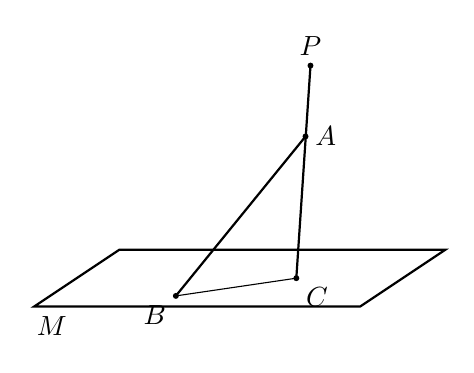
\begin{tikzpicture}[scale=0.9]
  % 地平面 M
  \draw[thick] (0,0) -- (4.6,0) -- (5.8,0.8) -- (1.2,0.8) -- cycle;
  \node[below] at (0.25,0) {$M$};
  % 电柱 PC：C 为柱脚，P 为柱顶，A 在 PC 上
  \draw[thick] (3.7,0.4) -- (3.9,3.4);
  \fill (3.9,3.4) circle (1.2pt) node[above] {$P$};
  \coordinate (A) at (3.83,2.4);
  \fill (A) circle (1.2pt) node[right] {$A$};
  \coordinate (C) at (3.7,0.4);
  \fill (C) circle (1.2pt) node[below right] {$C$};
  % 拉线 AB 与地面段 BC
  \draw[thick] (A) -- (2.0,0.15);
  \draw[thin] (C) -- (2.0,0.15);
  \fill (2.0,0.15) circle (1.2pt) node[below left] {$B$};
\end{tikzpicture}
